% Vietnamese translation for OI Public Library
% Source-PDF: IOI中国国家候选队论文/2000/江鹏论文.pdf
\documentclass[11pt]{article}
\usepackage{oipl-vn}
\usepackage{array}
\usepackage{booktabs}
\usepackage{tikz}
\usetikzlibrary{arrows.meta,positioning,calc,patterns}

\title{Khám phá các mô thức giải bài bằng phương pháp xây dựng}
\author{Jiang Peng}
\date{}

\newcommand{\problem}[1]{\subsection*{#1}}
\newcommand{\blankcell}{\phantom{$\bullet$}}
\newcommand{\filledcell}{$\bullet$}

\begin{document}
\maketitle

\origtitle{Exploring problem-solving patterns of the construction method}
\sourcepath{IOI China candidate team papers / 2000 / Jiang Peng.pdf}

\paragraph{Từ khóa.}
Phương pháp xây dựng; mô hình toán học.

\section*{Tóm tắt}

Bài viết thông qua một số ví dụ để khảo sát việc dùng phương pháp xây dựng
trong giải bài thi tin học. Trước hết bài viết trình bày cách vận dụng khéo
léo các phương pháp toán học, rồi đưa vào tư tưởng mô hình hóa toán học. Sau
đó bài viết thảo luận tương đối chi tiết cách xây dựng mô hình, gồm mô hình
trực tiếp xây dựng lời giải, mô hình đồ thị, mô hình luồng mạng và mô hình
tổ hợp. Bài viết giới thiệu phương pháp và mạch suy nghĩ cơ bản khi dựng mô
hình, đồng thời phân tích kiểu loại và tác dụng của mô hình toán học.

\renewcommand{\contentsname}{Mục lục}
\tableofcontents

\section{Dẫn nhập}

Giải bài bằng \term{phương pháp xây dựng} nghĩa là xây dựng một mô hình toán
học thích hợp để giải quyết vấn đề. Trong thi tin học, phương pháp này có
phạm vi ứng dụng rất rộng. Khi mô hình hoặc phương pháp được dựng đúng chỗ,
lời giải thường trở nên ngắn gọn và tinh tế.

Với những bài toán ta thường gặp, nếu phân loại theo phương pháp toán học thì
các mô hình được xây dựng chủ yếu thuộc hai nhóm: mô hình sơ cấp và mô hình
tối ưu hóa.

Nói chung, mô hình toán học có ba chức năng lớn.

\begin{enumerate}
  \item \term{Giải thích.} Dùng mô hình toán học để giải thích nguyên nhân
  của một hiện tượng.
  \item \term{Phán đoán.} Dùng mô hình toán học để đánh giá độ tin cậy của
  tri thức hoặc nhận thức ban đầu.
  \item \term{Dự báo.} Dựa trên tri thức, quy luật và chiều hướng phát triển
  được mô hình hóa để cung cấp chỉ dẫn hoặc tham khảo cho hành động.
\end{enumerate}

Mạch suy nghĩ khi giải bằng phương pháp xây dựng có thể khái quát như sau.

\begin{center}
\begin{tikzpicture}[>=Stealth,node distance=1.25cm]
  \tikzset{stage/.style={draw,rounded corners=2pt,minimum width=1.7cm,minimum height=.65cm}}
  \node[stage] (p) {Bài toán};
  \node[stage,right=of p] (h) {Giả thiết};
  \node[stage,right=of h] (m) {Mô hình};
  \node[stage,right=of m] (a) {Phân tích};
  \node[stage,right=of a] (i) {Hiện thực};
  \draw[->] (p) -- (h);
  \draw[->] (h) -- (m);
  \draw[->] (m) -- (a);
  \draw[->] (a) -- (i);
  \draw[->] ($(a.south)+(0,-.2)$) -- ++(0,-.7) -| node[pos=.25,below]{Kiểm nghiệm, sửa đổi} ($(m.south)+(0,-.2)$);
\end{tikzpicture}
\end{center}

Mục đích của bài viết này là dùng tư tưởng xây dựng mô hình toán học để xây
dựng lời giải cho các bài toán.

\section{Vận dụng khéo léo toán học}

Toán học nghiên cứu quan hệ số lượng và hình thức không gian của thế giới
hiện thực. Đặc điểm của toán học không chỉ nằm ở tính trừu tượng của khái
niệm, tính chặt chẽ của suy luận và tính xác định của kết luận, mà còn ở phạm
vi ứng dụng rất rộng. Nói đến phương pháp toán học là nói đến cách đơn giản
hóa và trừu tượng hóa một vấn đề phức tạp thành một cấu trúc toán học hợp lý.

Ta xét một số bài cụ thể để thấy các quan điểm ấy được vận dụng như thế nào.
Qua đó ta cũng thấy vai trò kỳ diệu của toán học và cảm nhận được niềm vui
khi giải bài bằng phương pháp toán học.

\problem{Bài toán 1: nhảy quân}

Cho một bàn cờ ô vuông $n\times n$ đã đặt kín quân. Quy tắc nhảy như sau.

\begin{enumerate}
  \item Khi một quân nhảy, ô kề nó theo cạnh phải có một quân khác làm quân
  đệm.
  \item Quân chỉ được nhảy theo phương ngang hoặc phương dọc.
  \item Quân nhảy qua quân đệm tới ô trống cùng hướng, rồi quân đệm bị lấy ra
  khỏi bàn.
\end{enumerate}

Mở rộng bàn cờ $n\times n$ thành bàn $m\times m$. Hãy tìm $m$ nhỏ nhất để các
quân có thể nhảy theo đúng quy tắc cho tới khi trong bàn chỉ còn một quân, và
hãy cho một phương án nhảy.

Nếu dùng tìm kiếm mù, ngay cả với $n=4,5$ cũng đã tốn kém. Ta thử giải bằng
xây dựng. Chia $n$ theo số dư khi chia cho $3$.

\paragraph{Trường hợp $n=3k$.}
Chia bàn $n\times n$ thành $k\times k$ khối $3\times 3$, rồi lặp mẫu tô màu
sau trên toàn mặt phẳng:

\[
\begin{array}{ccc}
1&2&3\\
2&3&1\\
3&1&2
\end{array}
\]

Mỗi lần nhảy luôn lấy hai màu này để đi tới màu còn lại. Gọi số lần nhảy tới
các màu $1,2,3$ lần lượt là $a,b,c$. Không mất tính tổng quát, giả sử quân
cuối cùng nằm trên màu $1$. Khi đó
\[
\begin{aligned}
3k^2+a-b-c &= 1,\\
3k^2-a+b-c &= 0,\\
3k^2-a-b+c &= 0.
\end{aligned}
\]
Lấy phương trình thứ nhất trừ phương trình thứ hai ta được
$2(a-b)=1$, mâu thuẫn vì $a,b$ là số nguyên. Do đó với $n=3k$ thì không thể
còn đúng một quân.

\paragraph{Trường hợp $n=3k+2$.}
Bắt đầu từ giá trị nhỏ để tìm quy luật. Với $n=2$ có thể giải bằng một khối
cơ sở $A$; ngoài ra ta dùng thêm hai khối cơ sở $B$ và $C$. Ba khối này có
tác dụng sau: với ba quân liên tiếp bất kỳ, nếu có thêm một quân phụ trợ thích
hợp thì có thể liên tiếp xóa ba quân ấy.

\begin{center}
\begin{tikzpicture}[scale=.55]
  \tikzset{cell/.style={draw,minimum size=.7cm}}
  \foreach \x in {0,1} \foreach \y in {0,1}
    \node[cell] at (\x,-\y) {};
  \node at (.5,-2) {$A$: khối $2\times2$};
  \begin{scope}[xshift=4cm]
    \foreach \x in {0,1,2,3} \node[cell] at (\x,0) {};
    \node at (1.5,-1.3) {$B$: dải ngang};
  \end{scope}
  \begin{scope}[xshift=9cm]
    \foreach \y in {0,1,2,3} \node[cell] at (0,-\y) {};
    \node at (0,-4.3) {$C$: dải dọc};
  \end{scope}
\end{tikzpicture}
\end{center}

Với $n=8$, ta đặt các khối cơ sở thành một sơ đồ: các hình vuông là khối
$A$, dải dọc là khối $C$, dải ngang là khối $B$. Trước hết xóa dải dọc phía
trên bên trái từ trái sang phải; sau đó xóa dải ngang phía trên bên phải từ
trên xuống dưới; cuối cùng lần lượt xóa các khối vuông và dải dọc phía dưới.

\begin{center}
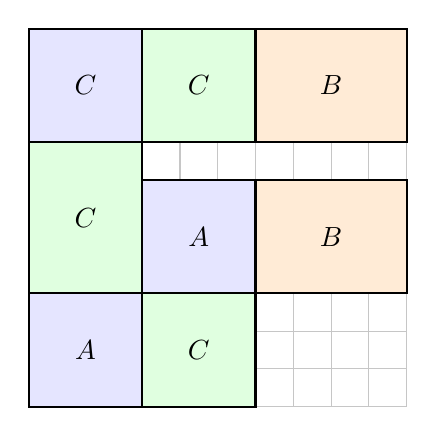
\begin{tikzpicture}[scale=.48]
  \draw[step=1,gray!45] (0,0) grid (10,10);
  \draw[thick,fill=blue!10] (0,7) rectangle (3,10);
  \draw[thick,fill=green!12] (3,7) rectangle (6,10);
  \draw[thick,fill=orange!16] (6,7) rectangle (10,10);
  \draw[thick,fill=green!12] (0,3) rectangle (3,7);
  \draw[thick,fill=blue!10] (3,3) rectangle (6,6);
  \draw[thick,fill=orange!16] (6,3) rectangle (10,6);
  \draw[thick,fill=blue!10] (0,0) rectangle (3,3);
  \draw[thick,fill=green!12] (3,0) rectangle (6,3);
  \node at (1.5,8.5) {$C$};
  \node at (4.5,8.5) {$C$};
  \node at (8,8.5) {$B$};
  \node at (1.5,5) {$C$};
  \node at (4.5,4.5) {$A$};
  \node at (8,4.5) {$B$};
  \node at (1.5,1.5) {$A$};
  \node at (4.5,1.5) {$C$};
\end{tikzpicture}
\end{center}

\paragraph{Trường hợp $n=3k+1$.}
Tương tự trường hợp trên, vẫn dùng các khối cơ sở để xây dựng. Với $n=7$, ta
xóa từng khối từ trên xuống dưới, từ trái sang phải; cuối cùng còn một hình
dạng như cán dao ở góc phải dưới, rồi xử lý riêng phần ấy.

Quan sát quá trình trên cho thấy chỉ cần mở rộng bàn cờ thêm một hàng ở mỗi
phía, tức biến thành bàn $(n+2)\times(n+2)$.

Bài toán này là một ví dụ điển hình của phương pháp xây dựng. Phương pháp
xây dựng không có khuôn cố định như tìm kiếm hay quy hoạch động; nó đòi hỏi
phân tích trạng thái, phân tích hình dạng và trừu tượng hóa theo tình huống
cụ thể. Vì vậy người giải cần nền tảng toán học tốt, năng lực sáng tạo và
tinh thần khoa học chặt chẽ.

\problem{Bài toán 2: ăn cơm quanh bàn tròn}

Có $n$ người ngồi quanh một bàn tròn. Không ai muốn trong hai ngày khác nhau
lại ngồi cạnh cùng một người. Hỏi nhiều nhất có thể sắp xếp được bao nhiêu
ngày, và hãy đưa ra một cách sắp xếp.

Để thấy rõ bản chất, mô tả bài toán bằng đồ thị. Cho $G=(V,E)$ là đồ thị đầy
đủ, $|V|=n$. Mỗi đỉnh biểu diễn một người, mỗi cạnh biểu diễn quan hệ ngồi
kề nhau. Mỗi cách ngồi quanh bàn trở thành một chu trình Hamilton của đồ thị.
Gọi $L=\langle v_1,v_2,\ldots,v_n\rangle$ là một chu trình Hamilton trong
$G$, và $e(L)$ là tập cạnh của nó. Cần tìm $m$ và
$L_1,L_2,\ldots,L_m$ sao cho $e(L_i)\cap e(L_j)=\varnothing$ với $i\ne j$,
đồng thời $m$ lớn nhất.

Trước hết ước lượng cận trên của $m$. Đồ thị đầy đủ có $n(n-1)/2$ cạnh, mỗi
chu trình Hamilton chứa $n$ cạnh, nên $m\le (n-1)/2$. Khi $n$ lẻ,
$m=(n-1)/2$; khi $n$ chẵn, $m=n/2-1$. Nếu xây dựng được đúng từng ấy chu
trình Hamilton rời cạnh thì cận trên này chính là đáp án.

Cách dựng như sau. Vẽ một đường tròn, chia đường tròn thành $n-1$ phần bằng
nhau, đánh dấu các đỉnh $1$ tới $n-1$ trên đường tròn, đặt đỉnh $n$ ở tâm.
Từ tâm nối tới một điểm tùy ý, rồi từ điểm đó lần lượt đi ngoằn ngoèo sang
hai phía trên đường tròn cho tới khi qua hết các điểm trên đường tròn, cuối
cùng nối về tâm. Ta được một chu trình Hamilton. Giữ nguyên vị trí đỉnh, quay
tất cả các dây nối quanh tâm ngược chiều kim đồng hồ một vạch; ta được chu
trình mới. Lặp phép quay $(n-1)\operatorname{div}2$ lần sẽ có
$(n-1)\operatorname{div}2$ chu trình.

\begin{center}
\begin{tikzpicture}[scale=.9]
  \foreach \ang/\lab in {90/4,162/5,234/1,306/2,18/3} {
    \coordinate (p\lab) at (\ang:1.6);
    \fill (p\lab) circle (1.6pt) node[shift={(\ang:.28)}] {\lab};
  }
  \fill (0,0) circle (1.6pt) node[below right] {6};
  \draw[gray!45] (0,0) circle (1.6);
  \draw[thick] (0,0)--(p1)--(p5)--(p2)--(p4)--(p3)--(0,0);
  \node at (0,-2.05) {$n=6$: một chu trình ban đầu};
  \begin{scope}[xshift=5cm]
    \foreach \ang/\lab in {90/4,162/5,234/1,306/2,18/3} {
      \coordinate (q\lab) at (\ang:1.6);
      \fill (q\lab) circle (1.6pt) node[shift={(\ang:.28)}] {\lab};
    }
    \fill (0,0) circle (1.6pt) node[below right] {6};
    \draw[gray!45] (0,0) circle (1.6);
    \draw[thick] (0,0)--(q5)--(q4)--(q1)--(q3)--(q2)--(0,0);
    \node at (0,-2.05) {Sau khi quay một vạch};
  \end{scope}
\end{tikzpicture}
\end{center}

Đúng đắn của cách dựng chỉ cần chứng minh các cạnh không bị trùng trong các
lần quay. Có thể chia cạnh thành hai loại: bán kính và dây. Dây lại được chia
theo độ dài thành $(n-1)\operatorname{div}2$ loại. Các cạnh khác loại hiển
nhiên không trùng khi quay. Trong cùng một loại, nhiều nhất có hai cạnh và
chúng nằm ở các vị trí đối nhau trong đường tròn, nên trước khi quay hết nửa
vòng chúng cũng không trùng.

Thuật toán có thể mô tả như sau.

\begin{verbatim}
Table(n):
  k <- 0; i <- 1; j <- n-1
  while i <= j:
    k <- k+1
    if k le:  r[k] <- i; i <- i+1
    else:     r[k] <- j; j <- j-1
  for shift <- 1 to (n-1) div 2:
    print ((r[t]-1+shift) mod (n-1))+1 for t=1..k
    print n
\end{verbatim}

\problem{Bài toán 3: con rết}

Con rết \emph{ishongololo} là một động vật chân đốt nhiều chân, thân dài,
màu đen bóng. Xét một khối hộp chữ nhật có chiều dài $K$, chiều rộng $W$,
chiều cao $H$ với các mặt đôi một vuông góc, $K,W,H\le 32$. Con rết bắt đầu
từ khối lập phương nhỏ $(1,1,1)$ và ăn sạch mọi khối trên đường đi. Các ràng
buộc chính là:

\begin{enumerate}
  \item Con rết luôn chiếm đúng một khối lập phương nhỏ rỗng.
  \item Mỗi lần nó ăn xong đúng một khối.
  \item Nó không được vào lại một khối đã từng đi qua.
  \item Nó không được đi vào khối chưa ăn và không được bò ra ngoài quả.
  \item Nó chỉ được ăn hoặc đi vào khối kề mặt với vị trí hiện tại; khối ấy
  còn phải không có mặt nào khác tiếp xúc với khối đã bị ăn sạch.
\end{enumerate}

Yêu cầu lập trình để con rết ăn được nhiều khối nhất có thể.

Đây là một bài của IOI 1997. Khó khăn thứ nhất là bài toán nằm trong không
gian ba chiều, đòi hỏi tưởng tượng hình học tốt; khó khăn thứ hai là trạng
thái phức tạp và số lượng trạng thái rất lớn. Tìm kiếm chỉ thích hợp để thăm
dò dữ liệu nhỏ. Đề gốc chấm điểm theo mức gần tối ưu, nhờ vậy bài toán bớt
khó hơn.

\paragraph{Đường đi phẳng.}
Trước hết xét trường hợp đơn giản $H=1$. Vì đường đã đi không thể đi lại,
cần tránh để đường đi quá sớm chia miền còn lại thành hai phần không còn liên
thông. Do đó tuyến chính nên đi theo kiểu uốn lượn.

Sau khi xác định tuyến chính, cần chọn khoảng cách giữa hai tuyến chính. Nếu
khoảng cách lớn hơn $2$ hàng thì sẽ có cả hàng trống không ăn được. Nếu cách
$1$ hàng, tuyến chính khá dày nhưng trên đường không ăn thêm được khối khác;
nếu cách $2$ hàng, tuyến chính chỉ chiếm khoảng một phần ba số hàng nhưng có
thể ăn xen kẽ thêm các khối hai bên. So sánh cho thấy cách $2$ hàng ăn được
xấp xỉ $2/3$ số khối, còn cách $1$ hàng chỉ khoảng $1/2$. Vì vậy dùng chiến
lược cách $2$ hàng.

\begin{center}
\begin{tikzpicture}[scale=.42]
  \draw[step=1,gray!35] (0,0) grid (10,6);
  \foreach \x in {0,...,9} {
    \fill[blue!30] (\x+.5,5.5) circle (.22);
    \fill[blue!30] (\x+.5,2.5) circle (.22);
  }
  \foreach \x in {1,3,5,7,9} {
    \fill[green!45] (\x-.5,4.5) circle (.18);
    \fill[green!45] (\x-.5,1.5) circle (.18);
  }
  \draw[very thick,->] (.5,5.5)--(9.5,5.5)--(9.5,2.5)--(.5,2.5);
  \node at (5,-.7) {Tuyến chính uốn lượn, giữa hai tuyến cách hai hàng};
\end{tikzpicture}
\end{center}

Khi so sánh với kết quả tìm kiếm trên mặt phẳng, lời giải xây dựng này khá
gần tối ưu.

\paragraph{Đường đi trong không gian.}
Lấy đường đi phẳng làm cơ sở để dựng đường đi ba chiều. Nếu con rết bò trong
mỗi lớp như sơ đồ phẳng thì kết quả sẽ rất tốt, nhưng khi nó đi qua một lớp,
một số khối ở lớp kề sẽ không còn ăn được. Cụ thể, sau khi khối $(x,y,z)$
bị ăn, nếu con rết tiếp tục đi trong mặt phẳng có tọa độ $z$, thì hai khối
$(x,y,z+1)$ và $(x,y,z-1)$ đều bị ảnh hưởng. Ảnh hưởng này không truyền cách
lớp: khối $(x,y,z)$ không ảnh hưởng tới lớp $z+i$ với $|i|>1$.

Vì vậy ta cho con rết di chuyển theo sơ đồ phẳng trên các lớp lẻ. Khi ở một
lớp lẻ đi từ một đỉnh tới đỉnh kia, nó đi lên và ăn hai khối để sang lớp lẻ
tiếp theo. Tạm thời chưa xét cách ăn ở lớp chẵn; các lớp lẻ khi đó không cản
trở nhau và đã tạo thành một lời giải khả thi.

\begin{center}
\begin{tikzpicture}[scale=.45]
  \foreach \z/\name in {0/Lớp 1,5/Lớp 2,10/Lớp 3} {
    \begin{scope}[xshift=\z cm]
      \draw[step=1,gray!35] (0,0) grid (4,4);
      \draw[very thick,blue!70] (.5,3.5)--(3.5,3.5)--(3.5,.5)--(.5,.5);
      \node at (2,-.6) {\name};
    \end{scope}
  }
  \draw[->,thick] (3.5,2) -- (5.5,2);
  \draw[->,thick] (8.5,2) -- (10.5,2);
\end{tikzpicture}
\end{center}

Nếu chỉ ăn ở các lớp lẻ, số khối ăn được khoảng $1/3$ tổng số. Ta còn có thể
ăn thêm ở lớp chẵn. Ở một lớp chẵn, những vị trí tương ứng với tuyến chính
của lớp lẻ bên trên và bên dưới đã bị hạn chế. Các khối của lớp chẵn chỉ nên
được ăn khi con rết đang đi trên tuyến chính của lớp $1$ hoặc lớp $3$. Khi đã
đến lớp $3$, việc ăn khối ở lớp $2$ không còn ảnh hưởng tới việc kéo dài
tuyến chính của lớp $3$, nên tại lớp $3$ nên ăn càng nhiều khối lớp $2$ càng
tốt. Như vậy tại khoảng $1/3$ số hàng của lớp chẵn có thể ăn xen kẽ khoảng
$1/2$ số khối; tính trên toàn khối hộp, ăn thêm khoảng $1/12$ tổng số. Tổng
cộng đạt xấp xỉ $1/3+1/12=5/12$.

\paragraph{Nhặt thêm trên đường.}
Trong các lớp lẻ ta không ăn lên lớp trên ngay từ đầu vì sợ cản trở tuyến
chính ở lớp cách hai tầng. Sau khi toàn bộ tuyến đã xác định, có thể từ lớp
lẻ ăn lên lớp kế tiếp nếu không ảnh hưởng tới tuyến đã định. Phần này lại
đem lại gần $1/12$ tổng số khối. Khi lập trình, nhờ tuyến chính đã cố định,
có thể kiểm tra điều kiện ăn khối và nhặt thêm nhiều nhất có thể.

Tới đây việc xây dựng cơ bản hoàn thành; phương pháp này ăn được khoảng một
nửa số khối.

\paragraph{Biến đổi tọa độ.}
Chiến lược trên dựa vào việc chọn một mặt đáy để làm mặt phẳng cơ sở. Khi
$K=W=H$, lựa chọn mặt đáy không quan trọng. Khi ba kích thước khác nhau, mặt
đáy ảnh hưởng tới số khối ăn được. Vì vậy ta thử cả ba cách chọn mặt đáy bằng
biến đổi tọa độ, qua đó cải thiện kết quả mà hầu như không tăng độ phức tạp
lập trình. Trong thử nghiệm, lựa chọn mặt đáy có thể làm kết quả khác nhau
tới khoảng $15\%$.

\section{Xây dựng một số kiểu mô hình}

Các ví dụ trên minh họa một kiểu dùng phương pháp xây dựng: trực tiếp xây
dựng lời giải của bài toán. Đây là kiểu đơn giản, chủ yếu dựa vào tính chất
riêng của từng bài, nên khả năng khái quát chưa cao. Muốn đi xa hơn và tìm
điểm chung của nhiều bài, cần nâng tư tưởng xây dựng lên mức mô hình hóa toán
học. Với các mô hình toán học trong phần này, ta chia theo tác dụng chính
thành hai nhóm lớn.

\begin{enumerate}
  \item \term{Mô hình để nhận thức sự vật.} Đây là trừu tượng của thế giới
  hiện thực. Nó rút ra thông tin hữu ích và biểu diễn bằng hình thức ngắn
  gọn: một công thức đại số, một hình hình học, một nguyên lý vật lý, một
  phương trình hóa học, thậm chí một hiện tượng tự nhiên. Bất cứ cấu trúc nào
  khái quát được sự vật khách quan và giúp mở rộng tư duy đều có thể thuộc
  loại này.

  \item \term{Mô hình để dẫn dắt thuật toán.} Loại này thường là một lý
  thuyết đã được nghiên cứu nhiều, có hệ tính chất và định lý phong phú. Trong
  thi tin học, các mô hình thường dùng gồm mô hình đồ thị, mô hình tổ hợp và
  mô hình luồng mạng. Chúng có nhiều thuật toán kinh điển để vận dụng, nên có
  vai trò quyết định trong thiết kế thuật toán.
\end{enumerate}

Sau đây là một số ví dụ về cách dựng và dùng các mô hình ấy.

\problem{Bài toán 4: xâu 01}

Cho $N,L_0,A_0,B_0,L_1,A_1,B_1$. Hãy thiết kế một xâu 01 độ dài $N$ sao cho
mọi xâu con liên tiếp độ dài $L_0$ có số ký tự $0$ nằm trong đoạn
$[A_0,B_0]$, và mọi xâu con liên tiếp độ dài $L_1$ có số ký tự $1$ nằm trong
đoạn $[A_1,B_1]$.

Đây là một bài trong NOI 1999. Trong kỳ thi, nhiều thí sinh dùng tìm kiếm sâu
kèm cắt nhánh theo biên; với $5$ bộ dữ liệu, thường giải đúng được $4$ bộ
trong thời gian cho phép. Nhìn lại, ta hỏi liệu có thuật toán đa thức gọn và
hiệu quả hay không.

\paragraph{Mô hình 4.1.}
Gọi xâu cần tìm là $S[1..N]$, $S[i]\in\{0,1\}$. Đặt $X[i]$ là số ký tự $1$
trong $i$ ký tự đầu của $S$, với $0\le i\le N$. Để $X[0..N]$ tương ứng với
một nghiệm của bài toán, cần có:

\[
X[0]=0,\qquad X[i-1]\le X[i]\le X[i-1]+1\quad (1\le i\le N).
\]

Với mọi xâu con độ dài $L_0$, số ký tự $1$ của nó là
$X[i+L_0]-X[i]$, nên điều kiện về số ký tự $0$ tương đương
\[
L_0-B_0\le X[i+L_0]-X[i]\le L_0-A_0\quad (0\le i\le N-L_0).
\]
Điều kiện về số ký tự $1$ trên độ dài $L_1$ là
\[
A_1\le X[i+L_1]-X[i]\le B_1\quad (0\le i\le N-L_1).
\]

Như vậy cần tìm một nghiệm nguyên của hệ bất đẳng thức trên. Nếu hệ vô
nghiệm thì bài toán gốc cũng vô nghiệm.

Mô hình 4.1 thuộc nhóm mô hình để nhận thức sự vật: nó viết lại đề bài bằng
ngôn ngữ hình thức ngắn gọn. Quan sát hệ điều kiện, ta thấy:

\begin{enumerate}
  \item trừ $X[0]=0$, các điều kiện còn lại đều là bất đẳng thức;
  \item mỗi bất đẳng thức chỉ chứa hai ẩn và một hằng số;
  \item có thể chuyển vế để đưa mỗi bất đẳng thức về dạng hai ẩn nằm ở hai
  phía, hệ số đều bằng $1$.
\end{enumerate}

Do đó mọi bất đẳng thức đều có thể viết thành
\[
X[i]+C\le X[j]\qquad (i,j=0..N).
\]
Dạng này gợi ta liên tưởng tới một cạnh có hướng nối hai đỉnh.

\paragraph{Mô hình 4.2.}
Dựng đồ thị có hướng $G$ gồm $N+1$ đỉnh, đánh số $0..N$. Với mỗi bất đẳng
thức $X[i]+C\le X[j]$, thêm cạnh có hướng $i\to j$ trọng số $C$.

Nếu $G$ không chứa chu trình dương, độ dài đường đi dài nhất giữa các đỉnh
tồn tại. Gọi $D[i]$ là độ dài đường đi dài nhất từ đỉnh $0$ tới đỉnh $i$.
Với mọi cạnh $i\to j$ trọng số $C[i,j]$, ta có
\[
D[i]+C[i,j]\le D[j].
\]
Nếu ngược lại thì đường đi từ $0$ tới $i$ rồi qua cạnh này tới $j$ sẽ dài hơn
đường đi dài nhất tới $j$, mâu thuẫn với định nghĩa của $D[j]$. Vì thế đặt
$X[i]=D[i]$ sẽ thỏa mọi ràng buộc.

Nếu $G$ chứa chu trình dương
$v_1\to v_2\to\cdots\to v_m\to v_1$ có tổng trọng số $C>0$, thì cộng các
bất đẳng thức trên chu trình thu được
\[
X[v_1]+C\le X[v_1],
\]
suy ra $C\le 0$, mâu thuẫn. Do đó hệ vô nghiệm.

Trường hợp không có chu trình dương có thể giải bằng lặp kiểu Bellman--Ford
cho đường đi dài nhất. Vì $X[i]$ chỉ tăng trong phạm vi hữu hạn, nếu sau $N$
vòng vẫn còn cập nhật thì tồn tại chu trình dương.

\begin{verbatim}
ZeroOneString:
  build graph G from all difference constraints
  X[0..N] <- 0
  k <- 0
  repeat:
    k <- k+1
    changed <- false
    for each edge i -> j with weight C:
      if X[i] + C > X[j]:
        X[j] <- X[i] + C
        changed <- true
  until not changed or k > N
  if k > N: report no solution
  else: print S[i] = X[i] - X[i-1]
\end{verbatim}

Trên thực tế đồ thị của bài này rất thưa: từ mỗi đỉnh nhiều nhất chỉ có vài
cạnh, nên không cần lưu ma trận kề. Dùng danh sách cạnh xuất phát từ mỗi đỉnh
sẽ hiệu quả hơn.

Toàn bộ lời giải gồm hai lần dựng mô hình. Lần thứ nhất chuyển đề bài thành
hệ bất đẳng thức; lần thứ hai chuyển hệ bất đẳng thức thành mô hình đồ thị.
Bản chất của quá trình xây dựng là liên tục biến bài toán gốc thành bài toán
tương đương mới, cho tới khi xuất hiện một bài toán dễ giải.

\problem{Bài toán 5: phân tách số nguyên}

Cho số nguyên $N$. Hãy đếm số cách tách $N$ thành $k$ số nguyên không âm nhỏ
hơn $n$, với $n>N/2$.

Bài toán chính là đếm số nghiệm của phương trình bất định
\[
X_1+X_2+\cdots+X_k=N,\qquad 0\le X_i\le n-1.
\]
Vì chỉ cần tổng số nghiệm, ta dùng hàm sinh.

Mỗi nghiệm tương ứng với hệ số của $x^N$ trong đa thức
\[
S=(1+x+\cdots+x^{n-1})^k.
\]
Đặt
\[
G=1+x+\cdots+x^{n-1}=\frac{1-x^n}{1-x},
\qquad S=G^k.
\]
Dùng khai triển
\[
(1+x)^m=\sum_{i=0}^{\infty}
\frac{m(m-1)\cdots(m-i+1)}{i!}x^i,
\]
ta có
\[
(1-x)^{-k}
=\sum_{i=0}^{\infty}\binom{k+i-1}{i}x^i.
\]
Do đó
\[
S=(1-x^n)^k(1-x)^{-k}.
\]
Vì $N<2n$, trong tích chỉ có thể nhận đóng góp từ hai hạng đầu của
$(1-x^n)^k=1-kx^n+\binom{k}{2}x^{2n}-\cdots$. Suy ra hệ số cần tìm là
\[
[x^N]S=
\begin{cases}
\binom{k+N-1}{N}, & N<n,\\[0.6em]
\binom{k+N-1}{N}-k\binom{k+N-n-1}{N-n}, & N\ge n.
\end{cases}
\]

Vì $n$ và $N$ có thể lớn, phần còn lại của chương trình là tính tổ hợp bằng
số nguyên độ chính xác cao. Ở đây mô hình hàm sinh biến bài toán đếm nghiệm
thành một công thức tổ hợp trực tiếp.

\section{Mô hình và thuật toán}

Dù trực tiếp xây dựng lời giải hay xây dựng mô hình toán học, điều ta quan
tâm nhất vẫn là thuật toán. Thiết kế được một thuật toán có độ phức tạp lập
trình thấp, độ phức tạp thời gian và bộ nhớ nhỏ, cấu trúc rõ ràng là mục tiêu
quan trọng. Có thể xét từ vài điểm sau:

\begin{enumerate}
  \item Mô hình được chọn phải thể hiện càng nhiều đặc trưng bản chất của bài
  toán càng tốt. Điều này không có nghĩa là mô hình càng phức tạp càng tốt;
  thông tin dư thừa sẽ làm giảm hiệu suất thuật toán.
  \item Việc dựng mô hình không diễn ra trong một bước, mà phải qua kiểm
  nghiệm và sửa đổi nhiều lần, rồi hoàn thiện dần trong thực hành.
  \item Mô hình toán học thường có hình thức nghiêm ngặt, nhưng khi hiện thực
  lập trình thì có thể linh hoạt.
\end{enumerate}

\problem{Bài toán 6: kinh doanh khách sạn}

Patiya là một thành phố du lịch đẹp. Mỗi kỳ nghỉ có rất nhiều du khách tới
Patiya. Khách sạn Royal Rose nằm bên bờ biển và có $R$ phòng. Trước kỳ nghỉ,
khách sạn nhận nhiều đơn đặt phòng từ các công ty du lịch, nhưng số phòng có
hạn nên không thể nhận tất cả. Giả sử bạn là quản lý khách sạn; hãy chọn nhận
một số đơn để lợi nhuận lớn nhất. Mỗi đơn cho biết thời điểm bắt đầu, thời
điểm kết thúc và số phòng đặt. Một khi nhận đơn, trong toàn bộ khoảng thời
gian ấy khách sạn phải cung cấp đủ phòng, nếu không sẽ mất uy tín.

\paragraph{Mô hình 6.1.}
Lập trục thời gian. Từ khi vị khách đầu tiên vào khách sạn tới khi vị khách
cuối cùng rời đi có $n$ ngày. Đánh số thời điểm bắt đầu ngày thứ nhất là
$1$, thời điểm giữa ngày thứ nhất và ngày thứ hai là $2$, và thời điểm kết
thúc ngày cuối là $n+1$. Mỗi đơn được biểu diễn bằng một đoạn thẳng có hai
đầu mút trên các điểm này. Gọi $c[i,j]$ là số đoạn có hai đầu mút $i,j$ với
$i<j$. Cần chọn một số đoạn sao cho trên mọi đoạn đơn vị của trục thời gian,
số đoạn phủ lên không vượt quá $R$, đồng thời tổng độ dài các đoạn đã chọn là
lớn nhất.

\begin{center}
\begin{tikzpicture}[>=Stealth,scale=.9]
  \draw[->] (0,0) -- (8,0);
  \foreach \x/\lab in {0/1,1/2,2/3,5.8/n,7/{n+1}} {
    \draw (\x,.08)--(\x,-.08) node[below]{\lab};
  }
  \draw[thick,blue!65] (0,.45)--(2,.45);
  \draw[thick,blue!65] (1,.85)--(5.8,.85);
  \draw[thick,blue!65] (2,1.25)--(7,1.25);
  \node at (4,-.75) {Các đơn đặt phòng là các đoạn trên trục thời gian};
\end{tikzpicture}
\end{center}

Mô hình này làm trạng thái rõ hơn. Một ý tưởng đầu tiên là tìm kiếm, chẳng
hạn lần lượt liệt kê số lần chọn từng đoạn. Nhưng tìm kiếm mù chỉ khai thác
bề mặt của bài toán và có độ phức tạp mũ.

Ta thử một thuật toán tham lam: lặp $R$ lần, mỗi lần chọn trong tập đoạn còn
lại một tập các đoạn đôi một không giao nhau sao cho tổng độ dài lớn nhất,
rồi xóa các đoạn ấy khỏi tập còn lại. Bước chọn tập đoạn không giao nhau dài
nhất có thể làm bằng quy hoạch động:
\[
D[1]=0,\qquad
D[i]=\max_{1\le j<i,\;c_0[j,i]>0}\{D[j]+i-j\},
\]
trong đó $c_0[j,i]$ là số đoạn $(j,i)$ còn lại.

Thuật toán này hấp dẫn nhưng không đúng tối ưu. Hình sau là một phản ví dụ:
lần đầu tham lam chọn các đoạn $1$ và $2$, lần hai chọn đoạn $4$, tổng độ dài
$12$; trong khi nghiệm tối ưu chọn cả bốn đoạn, tổng độ dài $14$.

\begin{center}
\begin{tikzpicture}[scale=.62]
  \draw[->] (0,0) -- (12.8,0);
  \foreach \x in {1,...,12} {
    \draw (\x,0.08)--(\x,-0.08) node[below]{\scriptsize \x};
  }
  \draw[very thick,blue!70] (1,1.2)--(6,1.2) node[midway,above]{1};
  \draw[very thick,green!55!black] (8,.9)--(12,.9) node[midway,above]{2};
  \draw[very thick,orange!80!black] (1,2.0)--(4,2.0) node[midway,above]{3};
  \draw[very thick,red!70] (4,2.6)--(12,2.6) node[midway,above]{4};
  \node at (6.5,-.9) {Một phản ví dụ cho tham lam theo từng lớp};
\end{tikzpicture}
\end{center}

Ta có thể sửa bước tham lam thành: trong lần thứ $I$, tìm tập đoạn $V$ sao
cho $A+V$ phủ mỗi đoạn đơn vị không quá $I$ lần và tổng độ dài của $V$ lớn
nhất. Nhưng các phản ví dụ tương tự vẫn tồn tại.

Qua việc thử tham lam, ta thấy quan hệ ràng buộc giữa các đại lượng khá phức
tạp; mô hình đồ thị thông thường khó mô tả. Vì vậy dùng mô hình luồng mạng.

\paragraph{Mô hình 6.2.}
Dựng mạng như sau.

\begin{enumerate}
  \item Tạo $n+1$ đỉnh đánh số $1$ tới $n+1$, biểu diễn các mốc trên trục
  thời gian; thêm nguồn $0$ và đích $n+2$.
  \item Với mỗi $I$, vẽ cung $I\to I+1$ có dung lượng vô hạn và chi phí $0$.
  \item Với mỗi đoạn $\langle I,J\rangle$, vẽ cung $I\to J$ có dung lượng
  $c[I,J]$ và chi phí bằng độ dài $J-I$. Lưu lượng trên cung này là số đơn
  loại ấy được nhận.
\end{enumerate}

Tìm luồng chi phí lớn nhất có giá trị $R$ trên mạng này; lưu lượng trên các
cung đơn đặt phòng chính là nghiệm của bài toán.

\begin{verbatim}
Hotel:
  build the flow network
  repeat R times:
    find a maximum-cost augmenting path
    augment along that path
  output booking arcs with positive flow
\end{verbatim}

Trong phản ví dụ trên, đường tăng luồng thứ nhất có thể đi qua các đoạn
tương ứng với lựa chọn tham lam ban đầu. Đường tăng luồng thứ hai được phép
dùng cung ngược của một đoạn đã chọn để điều chỉnh lại phương án, nhờ đó đạt
tổng chi phí $14$. Khác biệt bản chất giữa luồng cực đại chi phí và tham lam
nằm ở chính khả năng dùng cung ngược để sửa quyết định trước đó.

\section{Kết luận}

Xây dựng và mô hình hóa là một quá trình trừu tượng phức tạp. Ta cần nhìn
xuyên vào bản chất vấn đề, tìm điểm đột phá và chọn mô hình thích hợp. Mô
hình được xây dựng giúp ta nhận thức bài toán; các mô hình khác nhau phản
ánh bài toán từ các góc độ khác nhau, từ đó gợi ra nhiều hướng suy nghĩ.

Nhưng mục đích cuối cùng của nhận thức bài toán là giải bài toán. Tính chất
sẵn có của mô hình giúp ta thiết kế thuật toán; chất lượng thuật toán có thể
được đánh giá qua thời gian, bộ nhớ và các chỉ tiêu khác, nhưng cuối cùng vẫn
phải lấy chương trình hiện thực làm chuẩn. Vì vậy mô hình không bất biến; nó
cũng cần được tối ưu bằng nhiều kỹ thuật. Mô hình là sản phẩm của tư duy con
người, nhưng vẫn là phản ánh của sự vật khách quan trong tư duy ấy. Muốn có
năng lực mô hình hóa tốt, ta phải tích lũy tri thức và kinh nghiệm phong phú
trong học tập hằng ngày.

\section*{Tài liệu tham khảo}

\begin{enumerate}
  \item Fu Qingxiang, Wang Xiaodong. \emph{Thuật toán và cấu trúc dữ liệu}.
  \item Jiang Wenzai, chủ biên. \emph{Nhập môn Olympic Tin học}.
  \item \emph{Tạp chí Olympic Tin học}.
\end{enumerate}

\appendix

\section{Các đề bài được trích dẫn}

\subsection{Con rết}

Người Zulu gọi con rết là \emph{ishongololo}. Nó có thân dài, màu đen bóng,
là động vật chân đốt nhiều chân. Con rết ăn sạch mọi quả trên đường đi. Xét
một khối hộp chữ nhật kích thước $L\times W\times H$, với các mặt đôi một
vuông góc.

Chương trình cần xuất đường đi và hành động của con rết để nó ăn nhiều khối
nhất có thể. Con rết bắt đầu từ ngoài quả; khối đầu tiên bị ăn phải là
$(1,1,1)$, sau đó nó phải bò vào khối này và tiếp tục cho tới khi không còn
đường đi hoặc không còn khối hợp lệ để ăn.

Dữ liệu vào gồm ba số nguyên $L,W,H$, mỗi số trên một dòng, trong đoạn
$[1,32]$. Dữ liệu ra gồm nhiều dòng; mỗi dòng bắt đầu bằng \texttt{E} nghĩa
là ăn hoặc \texttt{M} nghĩa là di chuyển, sau đó là ba tọa độ của khối. Nếu
con rết vi phạm ràng buộc thì điểm bằng $0$; điểm nhận được tỉ lệ với số
khối đã ăn so với nghiệm tốt nhất đã biết, tối đa $100\%$.

\subsection{Xâu 01}

Cho bảy số nguyên $N,A_0,B_0,L_0,A_1,B_1,L_1$. Cần thiết kế xâu
$S=s_1s_2\ldots s_N$ sao cho $s_i$ là $0$ hoặc $1$; mọi xâu con liên tiếp
độ dài $L_0$ có số ký tự $0$ trong đoạn $[A_0,B_0]$; mọi xâu con liên tiếp
độ dài $L_1$ có số ký tự $1$ trong đoạn $[A_1,B_1]$.

Ví dụ với $N=6,A_0=1,B_0=2,L_0=3,A_1=1,B_1=1,L_1=2$, xâu
\texttt{010101} thỏa mọi điều kiện. Dữ liệu vào nằm trên một dòng, gồm bảy
số theo thứ tự trên. Nếu không có xâu thỏa điều kiện thì in \texttt{-1}; nếu
có thì in một xâu hợp lệ.

\section{Gợi ý hiện thực cho các bài toán}

\subsection{Nhảy quân}

Chương trình mô phỏng bàn cờ bằng mảng nhị phân, in trạng thái sau mỗi bước.
Ba thủ tục cơ sở tương ứng với khối $A$, dải ngang $B$ và dải dọc $C$ thực
hiện các chuỗi nhảy cố định. Nếu $n\bmod 3=0$ thì kết luận vô nghiệm. Nếu
$n\bmod 3=1$ hoặc $2$, chương trình lặp các thủ tục cơ sở theo từng khối
$3$ hàng hoặc $3$ cột, rồi xử lý riêng phần đuôi ở góc phải dưới.

\begin{verbatim}
Tiao(n):
  if n mod 3 = 0: report no solution
  fill the expanded board with pieces
  k <- n div 3
  if n mod 3 = 1: k <- k-1
  for full blocks: call vertical strip C
  for boundary rows: call horizontal strip B
  if n mod 3 = 1: handle the final handle-shaped part
  if n mod 3 = 2: handle the final 2x2 blocks
\end{verbatim}

\subsection{Xâu 01}

Hiện thực đọc dữ liệu, đổi điều kiện về số ký tự $0$ thành điều kiện về số
ký tự $1$, dựng các cạnh sai phân, rồi lặp nới lỏng đường đi dài nhất. Mỗi
đỉnh có số cạnh nhỏ, nên dùng danh sách cạnh xuất phát.

\begin{verbatim}
Construct:
  for i=1..N:
    add edge i-1 -> i with weight 0
    add edge i -> i-1 with weight -1
  for each window constraint:
    add edge left -> right with lower-bound weight
    add edge right -> left with negative upper-bound weight

Solve:
  D[0..N] <- 0
  repeat at most N+1 rounds:
    relax every edge that can increase D[v]
  if there is still an update after N rounds: print -1
  else print D[i]-D[i-1] for i=1..N
\end{verbatim}

\subsection{Khách sạn}

Mảng $a[i,j]$ lưu dung lượng của cung đơn đặt phòng từ ngày $i$ tới ngày
$j$. Mảng $f[i,j]$ lưu lưu lượng trên cung đơn đặt phòng; mảng một chiều lưu
lưu lượng trên các cung chuyển tiếp chi phí $0$. Mỗi vòng tìm đường tăng
luồng có chi phí lớn nhất bằng nới lỏng các cung thuận của đơn đặt phòng,
cung chuyển tiếp theo trục thời gian và cung ngược có lưu lượng dương. Sau
khi tìm được đường tới đích, lần ngược mảng cha để tăng hoặc giảm lưu lượng.

\subsection{Con rết}

Hiện thực dùng mảng ba chiều để ghi trạng thái từng khối:
$-1$ là vị trí đã đi qua, $-2$ là khối đã ăn, số không âm là số mặt đang lộ
ra với vùng đã ăn. Thủ tục \texttt{eat\_block} kiểm tra biên, kiểm tra số mặt
lộ ra, đánh dấu khối đã ăn và cập nhật các khối kề. Thủ tục \texttt{pick}
ăn thêm một khối kề nếu việc ăn đó chỉ chạm tuyến chính ở đúng một mặt.

Thủ tục dựng đường đi thử mọi hoán vị của ba trục tọa độ, sinh tuyến uốn
lượn trong các lớp lẻ, nối qua lớp chẵn, đồng thời nhặt thêm các khối hợp lệ.
Lần đầu chạy để chọn hoán vị tọa độ cho kết quả tốt nhất; lần sau chạy lại
với hoán vị ấy và in các lệnh \texttt{E} và \texttt{M}.

\end{document}
